\section{Software Maintainability} \label{chapter3:software-maintainability}

In order to improve and maintain a software system, it is important to holds in mind the mental representation behind its conception.
Architects, and mechanical engineers draw codified plans to share their mental representations with peers and building teams.
Similarly software developers write source codes.
But because the source code represents both the plan and its execution, the second aspect tends to shadow the first, and the mental representation is lost in technical details and optimizations.
It then becomes hard or even impossible to quickly grasp the purpose of the system without this mental representation.
Even the initial authors would have difficulties to understand the system after some times.
This problem becomes even more critical as the system grows in size.
Therefore, it is important to decompose the system into smaller subsystem easier to grasp individually.
Such decomposition improves the readability and comprehensibility hence maintainability of the implementation of a software system.
This section shows the theoretical tools for this decomposition, and their application in programming languages.


\subsection{Modularity}

\begin{center}
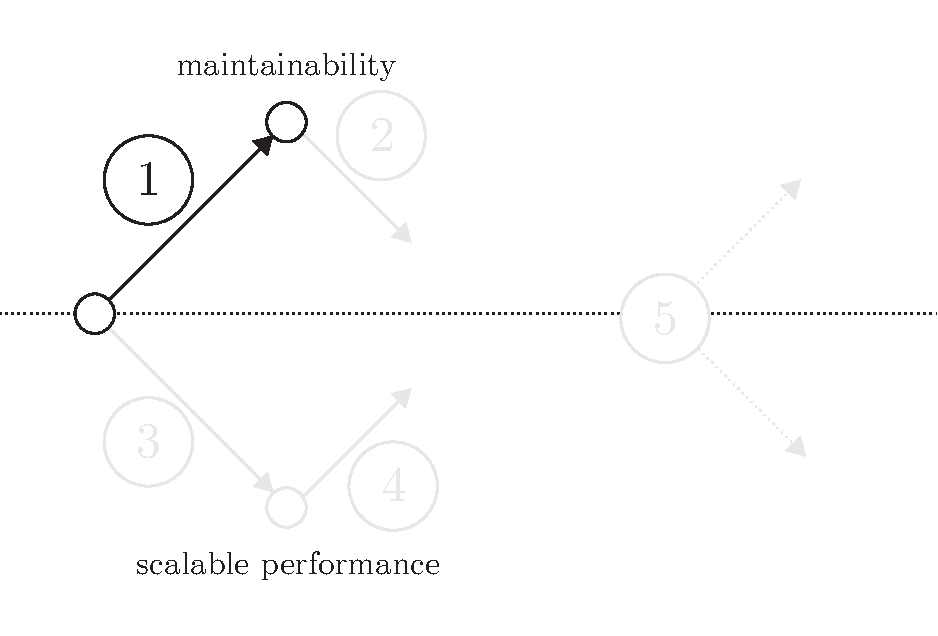
\includegraphics[width=0.6\textwidth]{../ressources/state-of-the-art-1.pdf}
\end{center}

\subsubsection{Design Choices}


\paragraph{Structured Programming}

\illustration{spaghetti programming}

The growing size and complexity of software systems eventually urges the developers to split the problem into isolated subproblems.
To respond to this problem, Dijkstra firstly developed the concept of Structured Programming \cite{Dijkstra1970}.
D. Knuth cited C. Hoare to define it as \textit{the systematic use of abstraction to control a mass of details, and also a means of documentation which aids program design} \cite{Knuth1974}.
Dijkstra formalized this procedure on two levels, at a fine grain and at a coarse grain \cite{Dijkstra1968a,Dijkstra1968}.

% A program expressed as a continuous flow of instructions with occasional jumps with 
The \texttt{goto} statement allows to jump anywhere in the code.
It makes the flow of control hard to follow and understand.
It is called spaghetti code.
Dijkstra advocated instead to decompose the implementation into structures and reusable functions to decompose the larger problem into many independent subproblems at a fine grain \cite{Dijkstra1968a}.
It is the precursor of many later programming trends.

\illustration{lasagna programming}

He also proposed to design complex systems with a hierarchical structure \cite{Dijkstra1968}.
It decomposes a system into layers at a coarser grain.
Each layer would abstract a design problem for the upper layers.
This work established grounds for what is know called modular programming.

% Letters to the editor : goto statement considered harmful \cite{Dijkstra1968a}
% The structure of the THE-multiprogramming system \cite{Dijkstra1968}

\paragraph{Modular Programming}

Modular programming advocates to design a software system as an assembly of modules communicating with each other.
The goal of using modular programming is twofold.
It allows to limit the understanding required to contribute to a module \cite{Stevens1974}.
% It allows a developer to limit its understanding only to the features isolated inside a module, instead of understanding the whole problem \cite{Stevens1974}.
And it reduces development time by allowing several developers to simultaneously implement different modules \cite{Wong2009,Cataldo2006}.

The criteria to decompose the system into well defined modules are coupling and cohesion \cite{Stevens1974}.
The coupling defines the strength of the interdependence between modules.
It is opposed to cohesion which defines how strongly the features inside a module are related.
Low coupling between modules and high cohesion inside modules imply a better readability and comprehensibility, hence a better maintainability of the implementation of the system.

These two criteria defines how modular is the implementation.
However, it doesn't define how well this organization will accept evolutions of the specification of the problem.
% stand against the evolution of the implementation.

% (See wikipedia page https://en.wikipedia.org/wiki/Separation_of_concerns)


\subsubsection{Design Choices}

The result of modular organization is that the modification on the implementation are easier to conduct within a module, than on the modules organization.
The impacts of the evolution of the problem should be concentrated as much as possible within the modules, and not in the modular organization, to reduce the overall impact on the implementation.
% It is important that the modular organization stand against the evolutions in the specification of the problem, and their consequences in the implementation.
% The interfaces between modules, and the contents of these modules need to be well thought.
The information hiding principle, and the separation of concerns are two similar approach to keep modifications within the modules.

\paragraph{Information Hiding Principle}

% helps define the content of modules so as to limit the impact of the evolution to a small portion of the implementation 
The information hiding principle advocates to encapsulate a specific design choice in each module to isolate the evolution on this choice from impacting the rest of the implementation \cite{Parnas1972}.
In this article, D. Parnas opposes the organization of modules following the information hiding principle from the one following a pipeline approach to parallelize the execution.
The former organization supports the development evolution, while the latter is more favorable to the performance of parallel execution.
This opposition shows that a program cannot trivially follow an organization that support both development evolution, and performance.
However, D. Parnas advocates the use of an assembler to conciliate the two approaches.

% The structure and value of modularity in software design \cite{Sullivan2001a}
% -> We identify an issue for software designers that neither Parnas’s formulation nor subsequent developments based on it adequately address: A designer is responsible for producing the greatest benefit for any given investment of time, talent, money, and other resources.

\paragraph{Separation of Concerns}

The Separation of Concern is a design principle advocating that each module is responsible for one and only one specific concern \cite{Tarr1999,Hursch1995}.
For example, the separation of the form and the content in HTML / CSS, or the OSI model for the network stack.
Each concern evolves independently without impacting the rest of the implementation.

However, this definition is orthogonal to the original meaning coined by Dijkstra \cite{Dijkstra1982}.
It is interesting to note this difference, as it is related directly to this thesis.
% Initially, it meant the ability to reason independently about different concern about a software system.
The initial definition was about analyzing independently how a system meets different concerns.
Dijkstra gives the example of analyzing independently correctness and efficiency.
It is impossible to encapsulate correctness, or efficiency in a module, they concern the whole system.
In this respect, this thesis is oriented towards dissociating the concern of development evolution and of performance.
That is to be able to reason on the maintainability of a program, independently than of its performance, and vice versa.
% This seems challenging as D. Parnas opposed these two concerns.
It is the challenge presented by D. Parnas when he opposed the two concerns in \cite{Parnas1972}.

This thesis investigates further this opposition to dissociate the concern of evolution and the concern of performance in the case of a web application.
The next section investigates the first concern, and presents the major programming models used to improve the evolution of an application.

\subsubsection{Programming Models} \label{chapter3:software-design:programming-models}

% Programming languages are designed for developers to follow the best practices mentioned above.
Programming languages used in the industry were designed following programming models favoring the use of the best practices mentioned above.
This section presents two programming models : object oriented programming and functional programming.

\paragraph{Object Oriented Programming}

% The following list defines Object-Oriented Programming (OOP).
% \begin{enumerate}
% \item Everything is an object.
% \item Communication is performed by objects communicating with each other, requesting that objects perform actions. Objects communicate by sending and receiving messages. A message is a request for action, bundled with whatever objects may be necessary to complete the task.
% \item Objects have their own memory, which consists of other objects.
% \item Every object is an instance of a class. A class simply represents a grouping of similar objects, such as integers or lists.
% \item The class is the repository for behavior associated with an object. That is, all objects that are instances of the same class can perform the same actions.
% \end{enumerate}

Alan Kay, who coined the term, states that Object Oriented Programming (OOP) is about message-passing, encapsulation and late binding.
(There is no academic reference for that, only a public mail exchange\ftnt{http://userpage.fu-berlin.de/~ram/pub/pub\_jf47ht81Ht/doc\_kay\_oop\_en}.)
This original definition is an evolution upon modular programming.
It helps encapsulate both the data, and the functions to process this data in an isolated, loosely coupled module.
The very first OOP language was Smalltalk \cite{Goldberg1984}.
It defined the core concept of OOP.
It is inspired by LISP and by the definition of the Actor Model, which we will define in the next section.

% Illustration of multiple cells, as Alan Kay thought of biology when developing the object-oriented concepts.
% http://userpage.fu-berlin.de/~ram/pub/pub_jf47ht81Ht/doc_kay_oop_en
% I thought of objects being like biological cells [...] able to communicate with messages ...

Object-Oriented Programming abandoned late-binding and adopted a stricter approach with the concepts of class, inheritance and polymorphism.
The major languages of the software industry feature this stricter Object-Oriented approach.
We can cite C++ and Java as the emblematic figures of OOP \cite{Gosling2000,Stroustrup1986}.

Though, the field test seems to have had reason of this stricter version.
The trends in programming language seems to digress from the pure Object-Oriented approach to evolve toward a more dynamic approach, closer to Functional Programming.
Indeed Javascript, Ruby and Python adopt functional features such as dynamic typing and higher-order functions \cite{Ecma1999}\ftnt{https://www.ruby-lang.org/en/about/}.

% \paragraph{Object Calisthenics}

% Object calisthenics are defined as the chapter 6 of \textit{The Thoughtworks Anthology} \cite{Bay2008}.
% It is an exercise for developers presented as a list of 9 rules to follow to enforce maintainability and readability on source code \ftnt{http://www.cs.helsinki.fi/u/luontola/tdd-2009/ext/ObjectCalisthenics.pdf}.

% Some of these rules are direct implementations of the more general concept of separation of concerns, and information hiding.
% As an example, rule 7 \textit{Keep all entities small} advocate that entities should have a concise concern.
% Other rules are just syntactic guides to improve readability and comprehensibility.


% See Object calisthenics 
% - http://williamdurand.fr/2013/06/03/object-calisthenics/
% - http://www.cs.helsinki.fi/u/luontola/tdd-2009/ext/ObjectCalisthenics.pdf



\paragraph{Functional Programming} \label{chapter3:software-design:programming-models:functional-programming}

% \cit{All problems in computer science can be solved by another level of indirection}{Butler Lampson}

The formal definition of Functional Programming resides in manipulating only mathematical expressions - instead of operation statements - and forbidding state mutability.
However, the functional programming concepts implemented in programming language are more mitigated, and resides in higher-order functions and lazy evaluation.
Two features that major programming languages now commonly present.
Higher-order functions and lazy evaluation help loosen the couple between modules, and improve their re-usability.
\textit{In fine}, it helps developers to write applications that are more maintainable, and favorable to evolution \cite{Hughes1989}.

\paragraph{Higher-Order Function}

Languages providing higher-order functions allows to manipulate functions like any other primary value : to store them in variables, or to pass them as arguments.
Higher-order functions replace the needs for most modern object oriented programming design patterns \ftnt{http://stackoverflow.com/a/5797892/933670}.

\paragraph{Closures}

Most languages use closures to implement lexical scope with higher-order functions \cite{Sussman1998}.
A closure is the association of a function and the lexical context from its creation.
It allows this function to access variable from this context, even when invoked outside the scope of this context.
For example when passed as an argument to another module.

It loosen the couple between modules, and helps define more generic and reusable modules.
However, it increase their dependencies during the execution.
Indeed, by exchanging closures, two modules intricately share their contexts of execution.

\paragraph{}

Functional programming greatly improves the resilience of implementation to the evolution of their specification.
However, it requires a global memory to share the context of execution among modules.
The next section shows that sharing memory makes parallelism difficult.
At the regard of this insight, the concern of evolution and the concern of performance seem hardly compatible.


\subsubsection{Higher-Order Programming}

\nt{TODO higher-order programming and modularity}

\subsubsection{Limitations}

\nt{TODO Transition on the limitations of software modularity}

\subsection{Performance Improvements}

\begin{center}
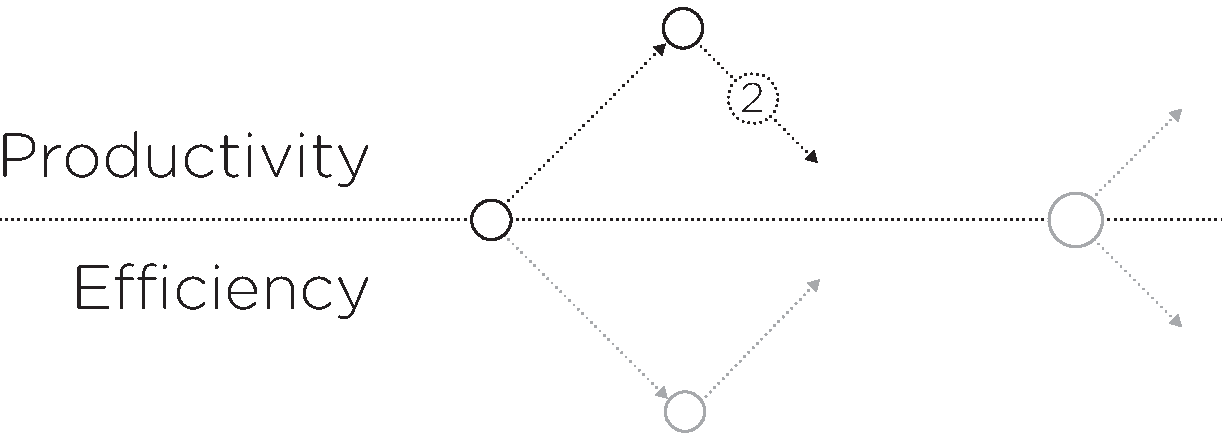
\includegraphics[width=0.6\textwidth]{../ressources/state-of-the-art-2.pdf}
\end{center}

\subsubsection{Compilation}


% Instead of trying to find a fitting between the two organization,
Another approach to conciliate performance and maintainability, is to transform the source from one organization into the other.
\textit{It is a mistake to attempt high concurrency without help from the compiler} \cite{Behren2003}.
When showing the incompatibility between the two organization, D. Parnas already advocated conciling the two methods using an assembler to transform the development organization into the execution organization \cite{Parnas1972}.
I present in the this section the state of the art in compilation-based parallelization.

% Imperative Stream Processing
%   Piccolo                                  Parallel in-memory \cite{Power2010}
%   CIEL                                    Stateless dataflow \cite{Murray2011}
%   Statdeful Dataflow Graph (SDG)          Stateful dataflow  \cite{Fernandez2014a}

\paragraph{Parallelism Extraction}

Generally, there is three type of parallelism, data, task and pipeline parallelism.
Some works explore the extraction of the three types indistincly \cite{Li2012}.
Other works focused on the task parallelism \cite{Rinard1996}.
However, huge works has been done on the data parallelization, to parallelize the loops inside a sequential program \cite{Mauras1989,Amarasinghe1995,Yuki2013,Banerjee2013,Radoi2014}
Indeed, the loops represent most of the execution time in scientific applications, so an important speedup is expected from this data parallelization.
C. Hermann studied the parallelization of loop in a functional language with higher-order programming and immutable data \cite{Herrmann2000}.
However, there is few works to parallelize higher-order programming languages, with mutable data.
Closures often complicates the dependencies between iterations.
To conserve higher-order programming, N. Matsakis proposed to forbid the mutation of the parent closure of a loop, so that the iterations can be executed in parallel while accessing the immutable closure\cite{Matsakis2012a}.

All these approaches are based on synchronous execution and Amdahl's law states that even if a slight portion of execution is sequential, the expected speedup is limited \cite{Amdahl1967,Clements2013a}.
Another approach to break free from the sequential structure is to split the sequential execution into following, parallelizable tasks to form a pipeline \cite{Kamruzzaman2013,Fernandez2014a}.
This thesis focus solely on pipeline parallelism.

Pipeline parallelism is relevant for multi-pass algorithms \cite{Conway1963}, and it is particularly efficient for stream processing applications as we saw in section \ref{chapter3:software-efficiency:dataflow-pipeline}.
For these applications, sequentiality is no longer relevant, as the different stages of the execution are repeated for each message in the stream.
Only causality is necessary, and it opens a possible pipeline parallelism.


\paragraph{Static analysis}

In order to extract parallelism, compilers analyze the source code of applications.
The compiler analyzes the control flow to detect the dependencies between statements to parallelize them.
As these dependencies are linked to memory access, it is important to have a good memory representation.
The point-to analysis, presented by L. Andersen \cite{Andersen1994} is a common approach to extract the memory representation.
It analyzes the modification of pointers through the control flow, to help extract properties from programs.
It is used in security to assure the safeness of an implementation, for example in Javascript \cite{Chudnov2015}.
% However, these techniques are not precise enough to rely only on them for the parallelization.

\paragraph{Annotations}

Extracting parallel dataflow from an imperative, sequential implementation is a hard problem \cite{Johnston2004a}.
Some works proposed to rely on annotations from the developer to help the extraction \cite{Vandierendonck2010a,Fernandez2014a}.
% Some works asked the developers to annotate their code so as help the compiler extract parallelism
% It is an intermediate solution with the solution presented in the previous section.
However, it still requires developers indicate the independence of the memory or the execution.
In this regard, this solution is similar to concurrent programming present in \ref{chapter3:concurrent-programming}, and are unable to fix the rupture between performance and maintainability.

All the solution presented throughout this chapter are elitist, as they tend to rely on the developer to reconcile the two organizations.
They are not satisfactory as they are too hardly accessible for most developers.
It finally results in frail implementations, that require great efforts of development to assure their performance in the first place, and then to maintain.

\subsubsection{Concurrent Programming}

\nt{TODO Event-loop / event-based programming / concurrent programming}

\begin{center}
\rule{3cm}{0.4pt}
need integration
\rule{3cm}{0.4pt}
\end{center}

\paragraph{Interdependencies}

It is easy to understand the parallelism in a cooking recipe because the interdependencies between operations are trivial.
It seems obvious that melting chocolate is independent from whipping up egg whites.
% Because chocolate and egg whites are different ingredients.
This distinction between chocolate and egg whites is trivial.
% ... comes from the modifications to the state.
While the distinctions within the state of an application are more intricate.
This makes concurrent application more difficult to design and implement.

\subparagraph{State Coordination}

% The interdependencies between the tasks impose the coordination of the global application state.
The global state of an application impose the coordination between the tasks.
This coordination happens either by sending messages, or by modifying a shared memory.
\nt{The following sentence needs to be rewritten to include both message passing and shared memory. Because state coordination limits parallelism, and scalability, it is a better solution to use message passing}
If the tasks are independent enough, the coordinations can be done with message passing.
Each task sends messages to indicate the modifications of the state with consequences outside its scope.
% They pass the states from one task to another so as to always have an exclusive access on the state.
% As example, applications built around a pipeline architecture define independent tasks arranged to be executed one after the other.
% The tasks pass the result of their computation to the next.
% These tasks never share a state.
However, if the tasks are too dependent, the overhead of message passing tends to impact performances.
% If the tasks need concurrent accesses to a state, they cannot efficiently pass the state from one to the other repeatedly.
They need to share and coordinate their accesses to the state.
Each access needs to be exclusive to avoid corruption.
I address in the next paragraphs the different scheduling strategies, and how they assure this exclusivity.

\subparagraph{Task Scheduling}

There are two scheduling strategies to execute tasks sequentially on a single processing unit : preemptive scheduling and cooperative scheduling.
The coordination is different with the two scheduling strategies.

\illustration{feu rouge et rond point}

Preemptive scheduling is used to assure fairness between the tasks, such as in a multi-tasking operating system.
% in most execution environment in conjunction with multi-threading.
The scheduler allows a limited time of execution for each task, before preempting it.
% It is a fair and pessimistic scheduling, as it grant the same amount of computing time to each task.
However, as the preemption happens unexpectedly, the developer needs to assure exclusivity by locking the shared state before access.
Locking is known to be hard to manage by developers, and to impact performances negatively.
Because it is not ideal both for development scalability and performance scalability, it is set aside for the remaining of this chapter.
% This scheduling strategy should be avoided except when true concurrency is needed in concert with true shared state.
% Shared state could probably always be emulated with isolated memory and message passing.

On the other hand, in cooperative scheduling, a task is allowed to run until it yields the execution back to the scheduler.
Each task is an atomic execution : it has an exclusive access on the memory.
% It gives back to the developer the control over the preemption.
As the developer doesn't need to explicitly assure exclusivity, it is easier to write concurrent programs efficiently with this scheduling strategy.
% Indeed, I presented in the previous section the popularity of Javascript, which is often implemented on top of this scheduling strategy (DOM, Node.js).

\subparagraph{Invariance}

\nt{TODO This section is not clear. It should be moved in the state of the art.}

% The challenge introduced above is to assure to the developer an exclusive access to the state of its application.
In concurrent computation, it is important to assure the invariance of a state during its manipulation.
This assurance is given by the exclusive access of an atomic execution on the state.
% I call invariance the assurance given that the state accessible from a task will remain unchanged during its access to avoid corruption, and more generally to allow the developer to perform atomic modifications on the state.
It allows the developer to group operations inside this atomic execution, so as to avoid corruption of the state.
% so as to perform all the operations without interference from concurrent executions.
% The same concept is found in transactional memory.

When the tasks remains isolated and communicate by message passing, there is no risk of corrupted state.
The invariance is assured by the isolation of the state specified by the developer, and by the atomicity of the message processing.
On the other hand, in a cooperative scheduling application, each task is atomic, so the developer always has an exclusive access to the global state.
This atomicity assures the invariance.
% The invariance is assured by the atomicity of each task.
% , because any region in the memory can be accessed only by one task at a time.

% Between these two invariances, the locking mechanisms seems to be a promising compromise.
% The developer defines only the shared states, and these are locked only when needed.
% However, it increases the complexity of the possible locked combination, leading to unpredictable situations, such as deadlock, and so on.
% The locking mechanisms are known to be difficult to manage, and sub-optimal.
% Indeed, they are eventually as efficient as a queue to share resources.

% For the rest of this thesis, I focus only on the invariances provided by the multi-process paradigm and the cooperative scheduling.
% They two invariance are similar, because the developer defines sequence of instructions with atomic access to the memory.
% And in both paradigms, these sequences communicate by sending messages to each other.
The difference is that in the message passing paradigm, the developer defines the state isolation inducing the execution isolation, while with cooperative scheduling, the developer defines only the execution isolation.
% This difference seems to be crucial in the adoption by the developer community.
It is difficult for developer to isolate state, but it provides good performances through parallelism.
While it is easier to assure atomic execution with cooperative scheduling, but it is unable to provide parallelism.
On one hand, the state is distributed and isolated to improve performance scalability.
On the other hand, the code is organized logically to improve maintainability.
The impact of these two organizations on performance scalability and development scalability is at the heart of this thesis.

\begin{center}
\rule{3cm}{0.4pt}
end integration
\rule{3cm}{0.4pt}
\end{center}


\subsubsection{Limitations on Accessibility}

\paragraph{Transition on parallel programming}

\endinput

\subsubsection{Modularity based on Design Decisions}

Designing Software for ease of extension and contraction \cite{Parnas1979}

Design Rules: The Power of Modularity Volume 1 \cite{Baldwin1999}
A reference book, but I can't get it.


Promises 
\cite{Liskov1988}


What makes a great software engineer? \cite{Li2015}

About great software development:
Productivity : Sackman et. al 68, Gugerty & Olson 86
Collaboration, meaningful contribution : Kelly 99, Begel & Simon 06, Hewner & Guzdial 10
Communicate and acquire understanding : LaToza 06, Ko 06
Technical Knowledge : 
Open minded : McConnell 04, Bryant 13




Modularity :
- encapsulation : a module contains the data, as well as the functions to manipulate this data
- separation of concerns : each module should have a clear scope of action, and this scope should not overlap with the scope of other modules
- loose coupling : each module should require no, or as little knowledge as possible about the definition of other modules






Continuations and coroutines \cite{Haynes1984}
-> THIS

Parallel closures, a new twist on an old idea \cite{Matsakis2012a}

Continuation of work on SEDA \cite{Salmito2014}



From control flow to dataflow \cite{Beck1991}


-> THIS, to read
Automatic Extraction of Coarse-Grained Data-Flow Threads from Imperative Programs \cite{Li2012}
In this paper all parallelism are extracted (data, task and pipeline).


Commutativity analysis: A new analysis framework for parallelizing compilers \cite{Rinard1996}
In this paper, they analyze commutative operations to parallelize them.
It is novel because it isn't about parallelizing loops.
However, it is not exactly pipeline parallelism either.


Interesting articles :

http://comjnl.oxfordjournals.org/content/early/2015/09/15/comjnl.bxv077.abstract


-> THIS, to read
Load balanced pipeline parallelism \cite{Kamruzzaman2013}


??? The Paralax infrastructure \cite{Vandierendonck2010a}

??? Blazes: Coordination analysis for distributed programs \cite{Alvaro2014}

Making state explicit ... \cite{Fernandez2014a}
http://2015.splashcon.org/event/splash2015-splash-i-lindsey-kuper-talk


Introducing 'Bones': a parallelizing source-to-source compiler based on algorithmic skeletons \cite{Nugteren2012}


Recent paper about Javascrypt static analysis \cite{Chudnov2015}



Loop nesting optimization
- systolic arrays
- polyhedral compilers
- Simplifying reductions 


\cite{Mendis2015}